\documentclass[12pt]{article}

% Opening
\title{Math 3012 Final Exam Part B}
\author{Akash Narayanan}

\usepackage{amsmath, amsfonts, amssymb, amsthm, enumitem, tikz}
\usepackage{caption, subcaption, float, marginnote, mathtools, mdframed}

% Solution environment
\newenvironment{solution}{
\begin{mdframed}
  { {\bfseries Solution}: }}{
\end{mdframed}}

\begin{document}

  \maketitle

  \begin{enumerate}
    \item (20 points) Consider the graph \textbf{G} shown below:

    \begin{figure}[H]
      \centering
      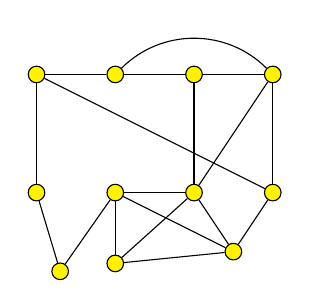
\begin{tikzpicture}
        [scale=1,every node/.style={draw,shape=circle,fill=yellow,inner sep=0,minimum size=6pt}, every draw/.style={line width=0.25mm, black}]

        \node (v1) at (0, 0) {};
        \node (v2) at (1, 0) {};
        \node (v3) at (2, 0) {};
        \node (v4) at (3, 0) {};
        \node (v5) at (0, -1.5) {};
        \node (v6) at (1, -1.5) {};
        \node (v7) at (2, -1.5) {};
        \node (v8) at (3, -1.5) {};
        \node (v9) at (0.3, -2.5) {};
        \node (v10) at (1, -2.4) {};
        \node (v11) at (2.5, -2.25) {};

        \draw (v1) -- (v2);
        \draw (v1) -- (v5);
        \draw (v1) -- (v8);
        \draw (v2) -- (v3);
        \draw (v2) to [out=45,in=135] (v4);
        \draw (v3) -- (v4);
        \draw (v3) -- (v7);
        \draw (v4) -- (v7);
        \draw (v4) -- (v8);
        \draw (v5) -- (v9);
        \draw (v6) -- (v7);
        \draw (v6) -- (v9);
        \draw (v6) -- (v10);
        \draw (v6) -- (v11);
        \draw (v7) -- (v10);
        \draw (v7) -- (v11);
        \draw (v8) -- (v11);
        \draw (v10) -- (v11);
      \end{tikzpicture}

    \end{figure}

    \begin{enumerate}[label=({\alph*})]
      \item (10 points) Find \(\omega(\textbf{G})\) for this graph. Show that \(\chi(\textbf{G}) = \omega(\textbf{G})\) by providing a proper coloring of \textbf{G}. You may indicate your coloring by writing directly on the figure.

      \item (10 points) Explain why the graph \textbf{G} is not perfect.
    \end{enumerate}

    \begin{solution}
      \begin{enumerate}[label=({\alph*})]
        \item \(\omega(\textbf{G})\) is the maximum clique size, and the largest clique in \textbf{G} has size 4.
        It is trivial that \(\chi(\textbf{G}) \geq \omega(\textbf{G})\), but we can see that the equality holds with the coloring shown below.

        \begin{figure}[H]
          \centering
          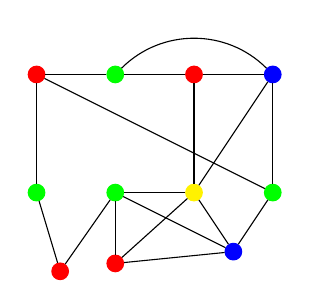
\begin{tikzpicture}
            [scale=1,every node/.style={draw,shape=circle,fill=yellow,inner sep=0,minimum size=6pt}, every draw/.style={line width=0.25mm, black}]

            \node[red] (v1) at (0, 0) {};
            \node[green] (v2) at (1, 0) {};
            \node[red] (v3) at (2, 0) {};
            \node[blue] (v4) at (3, 0) {};
            \node[green] (v5) at (0, -1.5) {};
            \node[green] (v6) at (1, -1.5) {};
            \node[yellow] (v7) at (2, -1.5) {};
            \node[green] (v8) at (3, -1.5) {};
            \node[red] (v9) at (0.3, -2.5) {};
            \node[red] (v10) at (1, -2.4) {};
            \node[blue] (v11) at (2.5, -2.25) {};

            \draw (v1) -- (v2);
            \draw (v1) -- (v5);
            \draw (v1) -- (v8);
            \draw (v2) -- (v3);
            \draw (v2) to [out=45,in=135] (v4);
            \draw (v3) -- (v4);
            \draw (v3) -- (v7);
            \draw (v4) -- (v7);
            \draw (v4) -- (v8);
            \draw (v5) -- (v9);
            \draw (v6) -- (v7);
            \draw (v6) -- (v9);
            \draw (v6) -- (v10);
            \draw (v6) -- (v11);
            \draw (v7) -- (v10);
            \draw (v7) -- (v11);
            \draw (v8) -- (v11);
            \draw (v10) -- (v11);
          \end{tikzpicture}

        \end{figure}

        \item A perfect graph is one in which \(\chi(\textbf{H}) = \omega(\textbf{H})\) for all induced subgraphs \textbf{H}.
        The graph \textbf{G} contains the following 7-cycle as an induced subgraph:

        \begin{figure}[H]
          \centering
          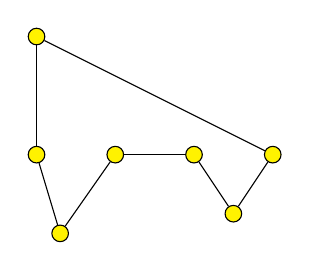
\begin{tikzpicture}
            [scale=1,every node/.style={draw,shape=circle,fill=yellow,inner sep=0,minimum size=6pt}, every draw/.style={line width=0.25mm, black}]

            \node (v1) at (0, 0) {};
            % \node (v2) at (1, 0) {};
            % \node (v3) at (2, 0) {};
            % \node (v4) at (3, 0) {};
            \node (v5) at (0, -1.5) {};
            \node (v6) at (1, -1.5) {};
            \node (v7) at (2, -1.5) {};
            \node (v8) at (3, -1.5) {};
            \node (v9) at (0.3, -2.5) {};
            % \node (v10) at (1, -2.4) {};
            \node (v11) at (2.5, -2.25) {};

            % \draw (v1) -- (v2);
            \draw (v1) -- (v5);
            \draw (v1) -- (v8);
            % \draw (v2) -- (v3);
            % \draw (v2) to [out=45,in=135] (v4);
            % \draw (v3) -- (v4);
            % \draw (v3) -- (v7);
            % \draw (v4) -- (v7);
            % \draw (v4) -- (v8);
            \draw (v5) -- (v9);
            \draw (v6) -- (v7);
            \draw (v6) -- (v9);
            % \draw (v6) -- (v10);
            % \draw (v6) -- (v11);
            % \draw (v7) -- (v10);
            \draw (v7) -- (v11);
            \draw (v8) -- (v11);
            % \draw (v10) -- (v11);
          \end{tikzpicture}

        \end{figure}
        Certainly for any odd cycle \textbf{C} larger than 3 we have \(\chi(\textbf{C}) = 3\) but \(\omega(\textbf{C}) = 2\).
        Therefore, \textbf{G} is not perfect because it contains an induced subgraph whose chromatic number is not equal to its maximum clique size.
      \end{enumerate}
    \end{solution}

    \pagebreak

    \item (20 points) Using induction, prove that for every positive integer \(n\),
    \begin{equation*}
      1 + 2 + \ldots + n = \frac{n (n+1)}{2}
    \end{equation*}

    \begin{solution}
      We begin with the base case of \(n = 1\). Certainly
      \begin{align*}
        1 = \frac{1 (1 + 1)}{2}
      \end{align*}
      Now suppose that the statement holds for some \(k \geq 1\). Then we have
      \begin{align*}
        1 + 2 + \ldots + k + (k + 1) &= \frac{k (k + 1)}{2} + (k + 1) \\
        &= \frac{k (k + 1)}{2} + \frac{2 (k + 1)}{2} \\
        &= \frac{(k + 1) (k + 2)}{2}
      \end{align*}
      That is, if the statement holds for \(k\) then it also holds for \(k + 1\).
      By the Principle of Induction, the statement holds for all integers \(n \geq 1\).
    \end{solution}

    \pagebreak

    \item (20 points)

    \begin{enumerate}[label=({\alph*})]
      \item (10 points) Find the general solution to the advancement operator equation:
      \begin{equation*}
        A^{4} (A - 5 + 4i)^{3} (A - 1)^{2} (A + 8) (A - 9) f = 0
      \end{equation*}

      \item (10 points) Find the solution to the advancement operator equation:
      \begin{equation*}
        (A^{2} - 11 A + 28) f(n) = 0, f(0) = -2, \text{ and } f(1) = 1
      \end{equation*}
    \end{enumerate}

    \begin{solution}
      \begin{enumerate}[label=({\alph*})]
        \item For the first equation, we use the fact that it is factored.
        We know that a basis for the solution space is given by functions of the form \(n^{i} r^{n}\) where \(r \neq 0\) is a root of the advancement polynomial and \(0 \leq m\) where \(m\) is the multiplicity of \(r\).
        Note that we exclude the root 0 because the basis function formed is simply 0 which is not linearly independent of the other functions.
        Using this, the general form of solutions to the recurrence equation is:
        \begin{align*}
          f(n) &= c_{1} (5 + 4i)^{n} + c_{2} n (5 + 4i)^{n} + c_{3} n^{2} (5 + 4i)^{n} \\
          &+ c_{4} + c_{5} n + c_{6} (-8)^{n} + c_{7} 9^{n}
        \end{align*}

        \item We start by factoring the advancement operator equation:
        \begin{equation*}
          (A^{2} - 11 A + 28) f(n) = (A - 7) (A - 4) f(n)
        \end{equation*}
        Then using the general theorem we know that the general form of solutions to the equation is:
        \begin{align*}
          f(n) = c_{1} 7^{n} + c_{2} 4^{n}
        \end{align*}
        Now we use the initial conditions to set up a system of equations.
        \begin{gather*}
          c_{1} + c_{2} = -2 \\
          7 c_{1} + 4 c_{2} = 1
        \end{gather*}
        Using elimination, we find that
        \begin{align*}
          3 c_{1} &= 9 \\
          \implies c_{1} &= 3
        \end{align*}
        Substituting this back into the top equation yields
        \(c_{2} = -5\).
        Therefore, the solution to the advancement operator equation is
        \begin{equation*}
          f(n) = 3 \cdot 7^{n} - 5 \cdot 4^{n}
        \end{equation*}
      \end{enumerate}
    \end{solution}

    \pagebreak

    \item (20 points) In a Bernoulli trial set up, there are three outcomes \(\xi_{1}\), \(\xi_{2}\), and \(\xi_{3}\) with probabilities \(p_{1}\), \(p_{2}\), and \(p_{3}\) respectively.
    The trial is repeated until either \(\xi_{1}\) occurs (this is a win) or \(\xi_{2}\) occurs (this is a loss).
    As long is \(\xi_{3}\) occurs, the trial is repeated. What is the probability of a win?

    \begin{solution}
      There are an infinite number of independent events resulting in a win so the probability of a win \(P\) is the sum of the probabilities of these events.
      \begin{align*}
        P &= p_{1} + p_{3} \cdot p_{1} + p_{3}^{2} \cdot p_{1} + p_{3}^{3} \cdot p_{1} + \cdots \\
        &= p_{1} \left(\frac{1}{1 - p_{3}}\right) \\
        &= \frac{p_{1}}{p_{1} + p_{2}}
      \end{align*}
      where we use the infinite geometric series from the first to second line (since \(p_{3} < 1\) it lies within the radius of convergence).
    \end{solution}

    \pagebreak

    \item (20 points)
    \begin{enumerate}[label=({\alph*})]
      \item (10 points) Write the inclusion/exclusion formula for the number of onto functions from \(\{1, 2, \ldots, n\}\) to \(\{1, 2, \ldots, m\}\).

      \item (10 points) Evaluate your formula when \(n = 6\) and \(m = 3\).
    \end{enumerate}

    \begin{solution}
      \begin{enumerate}[label=({\alph*})]
        \item The number of surjections from a set of size \(n\) to a set of size \(m\) is given by the formula
        \begin{equation*}
          S(n, m) = \sum_{k = 0}^{m} (-1)^{k} {m \choose k} (m - k)^{n}
        \end{equation*}

        \item Using the formula, we find
        \begin{align*}
          S(6, 3) &= \sum_{k = 0}^{3} (-1)^{k} {3 \choose k} (3 - k)^{6} \\
          &= 3^{6} - 3 \cdot 2^{6} + 3 \cdot 1^{6} - 0^{6} \\
          &= 540
        \end{align*}
        That is, given a set \(A\) of size 6 and a set \(B\) of size 3, there are 540 surjections from \(A\) to \(B\).
      \end{enumerate}
    \end{solution}
  \end{enumerate}
\end{document}
